\documentclass{article}
\usepackage[utf8]{inputenc}
\usepackage{dtk-logos} % for BibTeX stylized logo
\usepackage[english]{babel}
\usepackage[utf8]{inputenc}
\usepackage{algorithm}
\usepackage[noend]{algpseudocode}
\usepackage{amsmath,amsfonts,amsthm}
\usepackage[letterpaper, margin=1.25in]{geometry}
\usepackage{graphicx}
\usepackage{tabto}

\algnewcommand\algorithmicforeach{\textbf{for each}}
\algdef{S}[FOR]{ForEach}[1]{\algorithmicforeach\ #1\ \algorithmicdo}

\title{Selective Search: Partitioning Data into Shards for Lightweight Retrieval}
\author{Clayton Bond \\    
	    Computer and Information Sciences Department \\
	    University of Arkansas -- Fort Smith}
\date{\today}

\begin{document}
\maketitle

\begin{abstract}
	In this paper we go over some of the strengths and weaknesses of differing search techniques. What we're most interested in is developing a way to cluster a set of data to reduce the search time for each query. Selective Search will be our weapon of choice as it allows us to break down the data into shards via K-Means. We'll be comparing it against an older design that doesn't utilize cluster and instead relies on documents titles to narrow down the search term before preforming an exhaustive search.  stea
\end{abstract}

\section{Introduction}
In this paper we'll be detailing some of the steps that were taking to experiment with the effectiveness of Selective Search vs a less sophisticated but more personalized search technique for a small subset of Wikipedia data. The main methods tested were partitioning documents into topic clusters using Kmeans or putting more emphasis on document titles to create a what could be compared to a micro cluster. Both have strengths and weaknesses depending on your implementation. 

\section{Background}
Selective search is a modern distributed search architecture designed to reduce the computational cost of large-scale search. Selective search creates topical shards that are deliberately content-skewed, placing highly similar documents together in the same shard. My research was largely based off of the preceding work done by Yubin Kim and others at Carnegie Mellon University.  

\begin{quote}
Selective search architectures partition a document collection into
topic-oriented index shards, usually using algorithms that have
random components. Different mappings of documents into index
shards (\textit{shard maps}) produce different search accuracy and consistency, however identifying which shard maps will deliver the
highest average effectiveness is an open problem.

Selective search is a cluster-based distributed search architecture
that increases the efficiency of the early stages of a large-scale,
pipelined retrieval system. A large collection of D documents
is divided into n topically focused index shards. At query time, k
shards selected by a resource selection algorithm are searched,
typically k << n << D.
\end{quote}

\section{Specification}
During query time, rather than searching the entire corpus, a resource selection algorithm selects a subset of the topic shards likely to contain documents relevant to the query and search is only performed on these shards. This substantially reduces total computational costs of search while maintaining accuracy comparable to exhaustive distributed search. Prior work has shown selective search to be effective in smaller scale, single query-at-atime environments. However, modern practical, large-scale search and text analysis systems are often multi-stage pipeline systems where an initial, first-stage fast candidate retrieval forwards results onto downstream complex analysis components. 

\section{Implementation}

The first step in our program is to read in the data, to do this we call an external jar application that contains our tokenizer, stop words, spellcheck, and Tf-Idf. This is fed to our second step in preprocessing where we convert the data into a usable format for K-Means. 
\\\\
Once we feed the data to K-Means, we follow these steps to compute each cluster. 
\begin{itemize}
  \item Specify number of clusters K.
  \item Initialize centroids by first shuffling the dataset and then randomly selecting K data points for the centroids without replacement.
  \item Keep iterating until there is no change to the centroids. i.e assignment of data points to clusters isn’t changing.
  \item Compute the sum of the squared distance between data points and all centroids.
  \item Assign each data point to the closest cluster (centroid).
  \item Compute the centroids for the clusters by taking the average of the all data points that belong to each cluster.
\end{itemize}

After doing so, we pass these computed clusters to Naive Bayes to be narrowed down. This is how we perform our exhaustive search. Each cluster holds n documents that we compare to a target phrase. Inbetween these next steps a stochatic clustering method was also tested. Our implementation of Naive Bayes held to the following structure. 

$$C_{nb} = \textsc{argsmax  }logP(c) + \Sigma[logP(w_i|c)]$$
\begin{center}
Where $\hat{P}(c) = \dfrac{N_c}{N_{doc}}$
and $\hat{P}(w_i|c) = \dfrac{count(w_i,c)}{\Sigma_{w \in V} count(w,c)}$
\end{center}
This returned the greatest log probability for a cluster given a phrase.

\begin{algorithm}
\caption{"Naive Bayes"}
\begin{algorithmic}[Problem 1]
\State $classProb = log(N_c \div N_{doc})$
\ForEach{word $w$ in $vocabulary$}	
	\State $wordProb = wordProb +  log[(count(w|c) + 1) \div (count(w_i|c) + vocabulary)]$
\EndFor
\State \textbf{return}  $classProb + wordProb$
\end{algorithmic}
\end{algorithm}

The second tuned program to be used begins by loading in an ArrayList of all possible files we could be dealing with. These paths will be used to parse the page names and later to return to the file. To parse the page names, we simply grab the ending of the file right before the .html extension. 
\\\\
Now that everything is loaded, we search the page names and return the closest 100 matches to the phrase. This can be done by counting the amount of times a words occurs in a name. 

\begin{algorithm}
\caption{"Find Closest Names "}
\begin{algorithmic}[Problem 1]
\ForEach{word $w$ in $phrase$}	
	\ForEach{word $i$ in $path names$}
		\State count number of times $i$.contains$(w)$
	\EndFor
\EndFor
\end{algorithmic}
\end{algorithm}

\noindent
Once we have this, we can sort through and collect the top $x$ number of pages, in our case we used 100. We make $k*n$ passes through the file names. Where $k = $ number of words in the phrase. 

\begin{algorithm}[H]
\caption{"ReturnNames"}
\begin{algorithmic}[Problem 1]
\For{int $i = 0$ to number of files}	
	\If{k != -1}
		\If{file matches = k}
			\If{k= 0}
				\State No more items matching, fill the rest of the return with random guesses
			\EndIf
			\Else
				\State Add the name to the return
		\EndIf
		\If{$i = $ number of files}
			\State ReturnNames(k--)
		\EndIf
	\Else
		\State \textbf{return} names
	\EndIf
\EndFor
\State \textbf{return} names
\end{algorithmic}
\end{algorithm}

\noindent
Once this is done, we can pass these files to the tokenizer. This will clean out the majority of the html syntax to give us more usable data. A tokenizer isn't perfect though, so we'll be running it through a spell checker to help clean out anything that isn't a word. After this, we can clean even further by implementing TF-IDF to both remove any remaining html and improve our accuracy in Naive Bayes. 
\\\\
Finally, we return to evaluating with Naive Bayes.


\section{Evaluation}
There were a couple issues with my implementation. The first was difficulty in getting a standardized seed implemented to keep my results consistent. This meant that the cluster a search phrase was attached to had a random nature. However, I believe the results were blown out of proportion due to the closely related nature of the documents in my data set. The data is comprised mostly of STEM related articles with the majority being algorithms. If graphed, I would hypothesize that the result would be circular. Making it exceedingly difficult for K-Means to produce any meaningful results. 
\\\\
A method I took to circumvent this was to create a surplus of clusters in hopes that the clusters would have enough room to increase the accuracy. But the results were even more inaccurate by grouping the phrase with small index hmtl files that didn't provide any useful information gain. Though it would cost more time, I opted to keep the number of clusters lower to increase accuracy at the cost of efficiency.
\\\\
\textbf{Stochastic}
\begin{center}
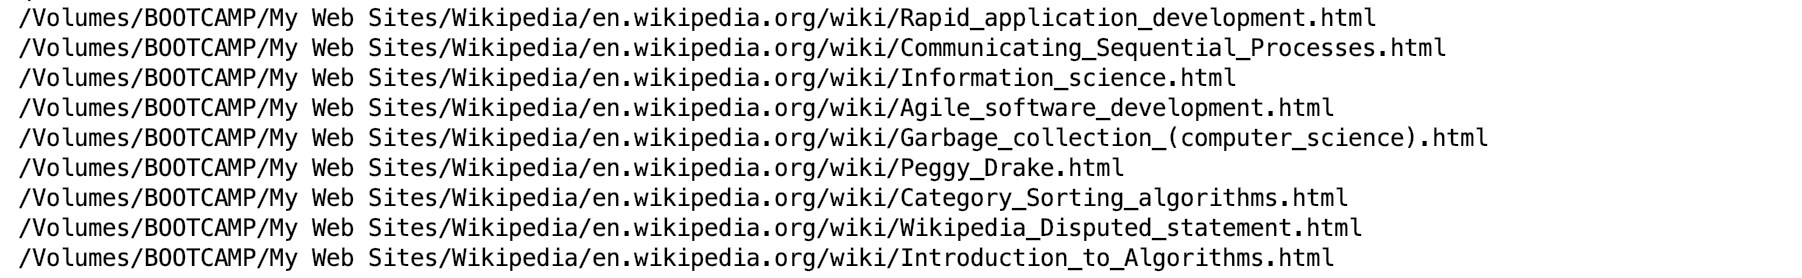
\includegraphics[scale=0.4]{Stochastic.png}\\
Success rate of $6.25\%$
\end{center}

Stochastic mathematically has a success rate of $6.25\%$ because it's assigning a cluster group randomly to two different entities, the desired document and the phrase. for both of these to be in the same group is a $25\%$ chance each (\textit{given 4 clusters}). Thus the chances that they both get assigned to the same group in a single run is $6.25\%$
\\\\
\noindent
\textbf{K-Means}
\begin{center}
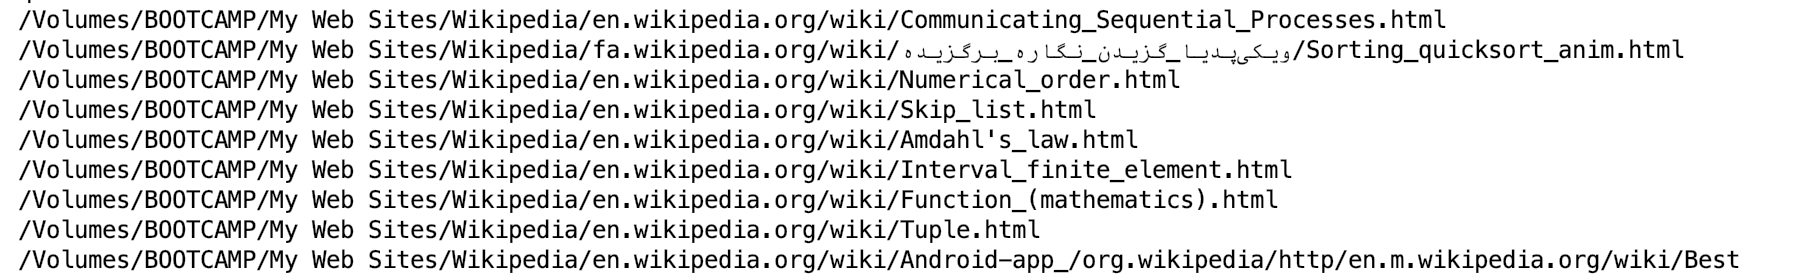
\includegraphics[scale=0.4]{Kmeans.png}\\
Success rate of $48.15\%$
\end{center}
K-Means had a success rate of roughly $48.15\%$. This is again due to the closely related nature of the data. Because we weren't able to generate meaningful clusters for more generalized terms like "XMOS" we ended up with search results that came up blank. for more specific terms like "HAL 9000" and "Douglas Adams" we were able to earn perfect marks

\begin{center}
    TensorFlow 2/1 \\
Shellsort 1/2 \\
Douglas Adams 3/0 \\
Personal Computer 0/3 \\
HAL 9000 3/0 \\
Xmos 0/3 \\
\end{center}

On the other hand, our homemade search system was able to achieve a modest $100\%$ success rate. However, this was a stacked test in it's favor. The terms listed above are the titles to their respective articles. which is at the core of it's design structure. When you implement something without a title into the test like "University of Russia". Then our tuned implementation is only able to find other Universities without anything relating to Russia. Our K-Means implementation on the other hand, was able to identify "Moscow State University" as it's more relationally based. This is a big win in favor of K-Means, as most searches are made with fragments of what we know. 
\\\\
An issue with the testing methodology we've taken in this paper is a lack of replicability. We weren't able to stabilize the seed which lead to random results. Even with a random seed you have the possibility to  leave the system running while you calculate the remaining queries. But this is a feature we weren't able to get running correctly. In the future there are a couple of additional steps we need to take to further test our results. First and most importantly we need to stabilize are search results. Second would be to perform a second web crawl on a similar data set and compare the success rate to what we already have. Third would be to bloat the data we already have, in theory this should increase the entropy in our data and increase our accuracy. 
\\\\
One final issue with this project was lack of scalability. When we create the clusters with K-Means, we're working with the entire corpus. That is we're scanning the entire file system and holding everything in a 2D array in memory. This could obviously have huge performance impacts. A better method would be creating a list holding a string of the filepaths. Only during the clustering process do you pull the file and preprocess it. This will leave you with a much smaller overhead with just two lists, one containing the list of filepaths and the other contain which group each filepath is associated with. 

\section{Conclusions}

For the simplicity of the data set the custom tuned application was the better option. But for bigger more stochastic sets I believe K-Means will come out on top. It's ability to search topical and relationally are much more powerful than returning a stagnate title. I believe a marrying of the two should be possible in a way that would substantially improve the performance of both algorithms in a huge data set. If K-Means was run first to cluster the data into meaningful shards then a seconds pass could be run over those shards using a title sweep to further narrow down the cluster, If this implementation took place an additional parameter would need to be added to the title search to increase the breadth of it's search to synonyms as well. 



\begin{thebibliography}{999}
\bibitem{Wachsmuth}
Wachsmuth, Henning, et al. “Building an Argument Search Engine for the Web.” ACL Anthology, \emph{Association for Computer Linguistics}, 25 Nov. 2018, aclanthology.coli.uni-saarland.de/papers/W17-5106/w17-5106.

\bibitem{Matsuo}
Matsuo, Yutaka, et al. “Graph-Based Word Clustering Using a Web Search Engine.” ACL Anthology, \emph{Association for Computer Linguistics}, 1 Dec. 2018, aclanthology.coli.uni-saarland.de/papers/W06-1664/w06-1664.

\bibitem{Saif}
Pham, Kim, et al. “Object Search: Supporting Structured Queries in Web Search Engines.” ACL Anthology, \emph{Association for Computer Linguistics}, 31 Nov. 2018, aclanthology.coli.uni-saarland.de/papers/W10-1206/w10-1206.

\bibitem{Kim}
Y. Kim, J. Callan, J. S. Culpepper, and A. Moffat, “Efficient distributed selective search,”Inf.Retr., vol. 20, no. 3, pp. 221–252, Jun. 2017. [Online]. Available: https://doi.org/10.1007/s10791-016-9290-6

\bibitem{Robust}
Y. Kim, “Robust selective search,”SIGIR Forum, vol. 52, no. 2, pp. 170–171, Jan. 2019.[Online]. Available: http://doi.acm.org/10.1145/3308774.3308803

\bibitem{Selective}
A. Kulkarni and J. Callan, “Selective search:  Efficient and effective search of large textualcollections,”ACM Trans. Inf. Syst., vol. 33, no. 4, pp. 17:1–17:33, Apr. 2015. [Online]. Available:http://doi.acm.org/10.1145/2738035

\bibitem{Measuring}
Kim, Yubin, Callan, and Jamie, “Measuring the effectiveness of selective search index partitionswithout supervision,” inProceedings of the 2018 ACM SIGIR International Conference onTheory of Information Retrieval, ser. ICTIR ’18.  New York, NY, USA: ACM, 2018, pp. 91–98.[Online]. Available: http://doi.acm.org/10.1145/3234944.3234952

\end{thebibliography}

\end{document}
